% Budget/contract: 0.95 page. Boundary section, not a selling-point section.
% Cover calibration with near-zero resolution, accuracy-based risk-coverage with no
% cost model or operating point, validation and guarded activity-tercile maps,
% guarded base rates, and label-shuffle sentinel. Activity means eligible-row count
% under the no-trade band, not volume/liquidity/volatility.
\section{Diagnostics and Robustness}
\label{sec:diagnostics}

This section reports two limits on the readouts. The confidence-based acceptance
signals of a near-base-rate classifier (calibration, selective prediction) are
largely illusory, and the thin edge inverts across activity terciles.

\paragraph{Calibration error is small, but resolution is near zero.}
On the frozen validation split, the pooled probability output has an equal-mass
ten-bin expected calibration error of approximately $0.010$. The Brier score is
$0.2496$, but its vector decomposition is dominated by the uncertainty term
($0.2499$), leaving a resolution component of about $4.7\times10^{-4}$
\cite{brier1950verification,murphy1973vector}. A small calibration error
therefore does not imply that the confidence scores rank cases usefully
\cite{guo2017calibration}.

\paragraph{Selective prediction barely beats random ranking.}
On the same validation split, the accuracy-based risk--coverage curve
(Figure~\ref{fig:risk_coverage}) carries no cost model and marks no operating
point. Its area (AURC) is approximately $0.470$ against an oracle value near
$0.140$, an excess area ($e$-AURC) of about $0.330$ in the seed mean. Read as
descriptive within-seed, day-level summaries, not seed-level estimates over
\numseeds{} seeds, the bands make the gain look thin.
Against the random-ranking reference the predeclared score lowers AURC only
marginally (\(\Delta\)AURC \(=-0.010\); \(95\%\) trading-day cluster-bootstrap CI
\([-0.014,-0.006]\)), about $3\%$ of the gap between random ranking and a
perfect-ranking oracle (gap-closed \(95\%\) CI \([1.9\%,4.0\%]\)). The gain
shrinks further at high coverage: the mean random-minus-score selective-risk
difference over the \(80\)--\(100\%\), \(90\)--\(100\%\), and \(95\)--\(100\%\)
bands is only \(0.25\), \(0.14\), and \(0.07\) percentage points. The companion
AUGRC is $0.237$
\cite{geifman2017selective,geifman2019selectivenet,elyaniv2010foundations,traub2024overcoming}.
To the extent low-confidence rows fall in the high-activity tercile, abstention
removes the classification rows where the below-random high-activity limitation
is most visible, and so compounds it \cite{chalkidis2021trading}.

\paragraph{Architectural-component ablation moves little (train-inner domain).}
One train-inner control precedes the conditional split. Here \texttt{tcn\_only} is
the primary's TCN and \texttt{dlinear\_only} is the hybrid's multi-scale DLinear
branch (MS-DLinear) with its residual TCN removed. Each control row's gap to
the reference stays within $\pm0.7\pp$ of \macrofone{} (\texttt{tcn\_only}
$+0.03\pp$, \texttt{dlinear\_only} $-0.14\pp$,
\texttt{last\_step\_lightgbm\_control} $-0.12\pp$, \texttt{last\_step\_mlp}
$-0.63\pp$; the latter two are last-step degenerate controls). The edge does not
turn on the control-row choice, and this control is never merged with the
validation or guarded readouts.

\paragraph{The edge concentrates in calm bars.}
We slice the same-row \macrofone{} delta by activity terciles---the
per-(ticker, trading-day) eligible-row-count proxy under the $3.0$ bps no-trade
band, not volume, liquidity, or volatility---rank-defined within ticker, so
there is no single global cut point. On the validation split the delta runs
$+5.43\pp$, $+1.91\pp$, and $-1.54\pp$ from low to high activity tercile
(Table~\ref{tab:tercile}). In the high tercile the \macrofone{} ($\approx
0.483$) sits below the even-class prior ($\approx 0.498$) and the same-row
stratified-dummy floor ($\approx 0.500$). The same direction recurs in the
guarded 2017--2024 era: $+4.08\pp$, $+0.56\pp$, and $-2.10\pp$, with a
high-tercile \macrofone{} of $0.480$ (Figure~\ref{fig:tercile_map}), the only
axis we could re-measure on the guarded segment. This is a non-independent
re-aggregation, not an independent replication. The figure's bars are
across-seed means with open circle/diamond seed markers; its grey sleeves are
per-trading-day block MDEs from official validation or measure-only
re-aggregation of frozen guarded dumps, not standard errors or seed-level
uncertainty. The signal is thus absent where the classifier faces the
hardest slice, the most active bars.

\begin{table}[t]
  \centering
  \caption{Activity-tercile condition map. Validation uses \numseeds{} seeds
  and guarded is non-independent. The high tercile falls below the
  balanced random prior in both domains; block-bootstrap checks are descriptive.
  Seed-mean rows (low/medium/high): 44{,}144/51{,}572/55{,}348 validation and
  95{,}310/111{,}178/119{,}479 guarded.}
  \label{tab:tercile}
  \begin{tabular}{lrr}
    \toprule
    Activity tercile & Validation $\Delta$ & Guarded $\Delta$ \\
    \midrule
    Low activity    & $+5.43\pp$ & $+4.08\pp$ \\
    Medium activity & $+1.91\pp$ & $+0.56\pp$ \\
    High activity   & $-1.54\pp$ & $-2.10\pp$ \\
    \midrule
    High-tercile \macrofone{} & $\approx 0.483$ & $0.480$ \\
    Balanced prior & \multicolumn{2}{c}{$\approx 0.498$--$0.500$} \\
    \bottomrule
  \end{tabular}
\end{table}

\paragraph{Base-rate and within-day artifacts are excluded, but a microstructure artifact is not.}
The one alternative our controls cannot exclude is microstructure: the calm-bar
concentration cannot presently be separated from a bid-ask-bounce alignment, and
the sentinel has no power to do so. The bounce is a true row-level feature--label
coupling that a within-day permutation preserves
\cite{roll1984simple,lo1990nonsynchronous}, and the discriminating control needs
raw five-minute bars the dump does not carry. The near-constant per-tercile dummy
floor ($\approx 0.500$) rules out a class-imbalance artifact, while the up-rate
shows only a small monotone gradient ($0.523$, $0.515$, $0.502$ from low to high,
about $2.1\pp$). A fifty-permutation within-day label-shuffle sentinel rules out
within-day leakage. The observed delta exceeds the per-tercile shuffle maximum in
every tercile, including the high tercile. There it exceeds a more negative
shuffle null while staying below random. So the below-random value is itself not a
permutation artifact. Because this confound remains open, we report
the map as a diagnostic boundary on this estimand, not as model-attributable
conditional predictability. If model-attributable it would run against prior
intraday-return work tying short-horizon predictability to intraday timing,
higher-activity states, or seasonal rebalancing
\cite{heston2010intraday,henkel2011timevarying,bogousslavsky2016infrequent}.
A recent regime study does report forecastability in low-financial-uncertainty
periods \cite{ferrer2023forecast}, a regime-level parallel, not one at our
resolution. We carry the deferred microstructure control as a limitation
(Section~\ref{sec:limitations}).

\begin{figure}[t]
  \centering
  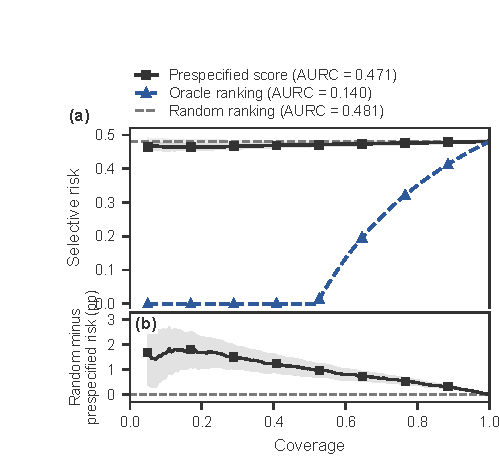
\includegraphics[width=0.92\linewidth]{figures/fig_risk_coverage}
  \Description{A two-panel accuracy-based selective-risk--coverage diagnostic.
    The top panel shows selective risk against coverage: the predeclared
    confidence-score curve stays close to the expected-random-ranking reference,
    while a dashed perfect-ranking oracle lies much lower. The lower panel shows
    the expected random-ranking risk minus the predeclared score risk in
    percentage points, staying near zero across most coverages. Light bands show descriptive
    trading-day cluster-bootstrap and random-ranking permutation intervals. The chart shows
    accuracy only, with no cost model and no chosen operating point.}
  \caption{Accuracy-based selective-risk--coverage diagnostic; lower is better.
  The curve barely separates from random ranking, indicating weak confidence
  ordering rather than a usable abstention rule. There is no chosen operating
  point; with \numseeds{} training seeds, the plot establishes no statistical
  significance, calibration, or deployable abstention policy.}
  \label{fig:risk_coverage}
\end{figure}

\begin{figure}[H]
  \centering
  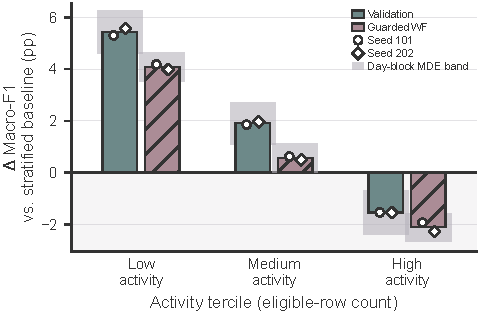
\includegraphics[width=0.85\linewidth]{figures/fig_tercile_map}
  \Description{A grouped diverging bar chart with activity terciles on the
    horizontal axis and macro-F1 differences over the same-row stratified dummy
    on the vertical axis, in percentage points. Each tercile has two bars:
    validation and guarded walk-forward. Open circle and diamond markers overlay
    the two seed-specific values. A bold horizontal zero line marks the dummy
    floor, and a faint grey band below zero marks negative differences. Faded
    grey rectangles around bar endpoints show the day-block minimum detectable
    effect. The bars decline from the low- to high-activity tercile, and the
    high-activity bars are below zero in both domains.}
  \caption{Activity-tercile condition map. Paired diverging bars compare validation
  and guarded \macrofone{} deltas over the same-row stratified dummy; positive
  values favor the model. Activity is an eligible-row-count proxy under the
  no-trade band, not volume, liquidity, or volatility. The high-activity
  inversion is a limitation; guarded results are non-independent, not a
  clean test, and grey sleeves are not confidence intervals.}
  \label{fig:tercile_map}
\end{figure}
